\documentclass[authoryear,review, 12pt]{elsarticle}



\newcommand{\maxwidth}{\textwidth}

\usepackage{alltt}
\usepackage[T1]{fontenc}
\usepackage[latin9]{inputenc}
\usepackage{geometry}
\geometry{verbose}
\setlength{\parskip}{\medskipamount}
\setlength{\parindent}{0pt}
\usepackage{bm}
\usepackage{amsthm}
\usepackage{amsmath}
\usepackage{amssymb}
\usepackage{undertilde}
\usepackage{graphicx}
\usepackage{setspace}
\usepackage{esint}
\usepackage{booktabs}
\usepackage{color}
\usepackage{multirow}
\usepackage{natbib}
\usepackage{ifthen}

\mathchardef\mhyphen="2D % Define a "math hyphen"

\newcommand{\hlc}[2][yellow]{ {\sethlcolor{#1} \hl{#2}} }
\newcommand{\highlight}[1]{\colorbox{yellow}{$\displaystyle #1$}}

\newtheorem{thm}{Theorem}
\newtheorem{lem}{Lemma}

\newcommand\pr{\mathbf P}
\newcommand{\E}{\mathbb{E}}

\setlength{\textwidth}{6.5in}
\setlength{\textheight}{8.5in}
\textwidth=6.5in
\textheight=8.5in
\setlength{\topmargin}{0in}
\setlength{\oddsidemargin}{0in}
\setlength{\evensidemargin}{0in}

\journal{ASA Student Paper Competition - Nonparametric Section}

\newboolean{thesis}
\setboolean{thesis}{false}

\begin{document}


\begin{frontmatter}

\title{Local Adaptive Grouped Regularization and its Oracle Properties for Varying Coefficient Regression}


\author[wrbrooks]{Wesley Brooks}
\ead{wrbrooks@uwalumni.com}

\address[wrbrooks]{Department of Statistics, University of Wisconsin, Madison, WI 53706}

\end{frontmatter}
\vspace{-4em}

\section{Introduction}

Whereas the coefficients in traditional linear regression are scalar
constants, the coefficients in a varying coefficient regression (VCR)
model are functions - often \emph{smooth} functions - of some effect-modifying
parameter \citep{Hastie-Tibshirani-1993}. Here
we treat the case of a VCR model on a spatial domain where the spatial
location is a two-dimensional effect-modifying parameter. Current
practice for VCR models relies on global model selection by, for example, basis expansion \citep{Wang-2008a}, or
local regression \citep{Wang-Xia-2009}. Since the coefficients vary
in a VCR model, it is natural to allow that the set of relevant covariates may vary over the domain.

This paper introduces local adaptive grouped regularization (LAGR)
for local variable selection and estimation in VCR model. The method of LAGR applies to VCR models
where the coefficients are estimated using locally linear kernel smoothing.
Kernel smoothing for nonparametric regression is described in detail
in \citet*{Fan-Gijbels-1996}. The extension to estimating VCR models
is made by \citet{Fan-Zhang-1999}. These methods mitigate the boundary effect by
estimating the coefficients as local polynomials of odd degree (usually
locally linear) \citep{Hastie:1993b}.

The adaptive Lasso (AL) is a regularization method that
simultaneously selects covariates for a regression model and shrinks
the coefficient estimates toward zero \citep{Zou-2006}. The AL has been shown to have appealing properties for
variable selection, which under suitable conditions include the ``oracle''
property of asymptotically including exactly the correct set of covariates
and estimating their coefficients as well as if the correct covariates
were known in advance \citep{Zou-2006}. For data where the observed
covariates fall into mutually exclusive groups that are known in advance,
the adaptive group Lasso has similar oracle properties to the adaptive
Lasso but selects groups rather than individual covariates
\citep{Yuan-Lin-2006,Wang-Leng-2008}. The method of LAGR uses an adaptive group Lasso that achieves the oracle properties in the local regression setting, where convergence is slower than the typical $n^{1/2}$ rate.

The remainder of this paper is organized as follows. The kernel-based
estimation of a VCR model is described in Section \ref{sec:vcr}.
The proposed LAGR technique for varying coefficient linear regression
and its oracle properties are presented in Section \ref{sec:lagr-gaussian}.
In Section \ref{sec:example},
LAGR is applied to the Boston housing price dataset, followed
by conclusions and discussion in Section 5. Technical proofs are given in the Appendix.

\section{Varying Coefficient Regression\label{sec:vcr}}
Throughout the paper, we work with the generalized linear model (GLM) \citep{McCullagh-Nelder-1989}. The response of a GLM can come from any distribution in the exponential family, so the familiar linear regression model is included as a special case.

\subsection{Varying coefficient model}
The response $Y(s)$, covariates $\bm{X}(s)$, and coefficients $\bm{\beta}(s)$ in a VCR model are indexed by the location parameter $s$. Let $d$ be the dimension of the location parameter (e.g., $d=1$ for a coefficients that vary with time). Assume $n$ observations of the response and the covariates at locations $s_1, \dots, s_n$ and let $Y_i = Y(s_i)$, $\bm{X}_i = \bm{X}(s_i)$, and $\bm{\beta}_i = \bm{\beta}(s_i)$. The generalized linear model (GLM) with varying coefficients is written
\begin{align*}
	E[Y(s)|\bm{X}(s)] &= \mu(s)\\
	\eta(s) = g(\mu(s)) &= \bm{X}'(s) \bm{\beta}(s)\\
	\text{var}[Y(s)|\bm{X}(s)] &= \phi V(\mu(s))
\end{align*}
where $g(\cdot)$, $V(\cdot)$, and $\phi$ are, respectively, the link function, variance function, and dispersion parameter of the response family. For simplicity of notation, assume the canonical link function.

\subsection{Local polynomial regression}
In the context of nonparametric regression, the boundary-effect bias
can be reduced by local polynomial modeling, usually in the form of
a locally linear model \citep{Fan-Gijbels-1996}. Near estimation location $s$, the coefficient functions are well approximated by Taylor's expansion as locally linear functions of the location parameter
\begin{equation}\label{eq:taylors}
\bm{\beta}(t) = \bm{\beta}(s) + \nabla \bm{\beta}(s) (t - s) + o(|t - s|).
\end{equation}
The locally linear approximation is implemented by augmenting the matrix $\bm{X}$ with interactions between the covariates and the location parameter. Let the augmented covariates be $\bm{Z}(s) = \left( \bm{X}_i \;\; \text{diag}\{s-s_i\}_{i=1}^{n} \cdot\bm{X}_i \right)$ and the augmented coefficients be $\bm{\zeta}(s) = (\bm{\beta}(s)^T, \; \nabla \bm{\beta}(s)^T)^T$.
%, the linear predictor of the local GLM is $\hat{\eta}_i = \bm{Z}_i \hat{\bm{\zeta}}_i$.

\subsection{Coefficient estimation via local quasi-likelihood}
The quasi-likelihood $Q(\mu, Y)$ is an approximation to the log likelihood. Its derivative the quasi-score function is $q(\mu, Y) = (y-\mu) \{V(\mu)\}^{-1}$, which is a function of the linear predictor $\eta$ through the link and variance functions. Taylor's approximation \eqref{eq:taylors} is more accurate nearer to $s$, so a kernel function $K_{h}(\|s-s_{i}\|) = h^{-d} K(h^{-1} \|s - s_i \| )$ is used to weight the observations based on their distance from $s$ and the bandwidth parameter $h$. For instance, the Epanechnikov kernel is:
\begin{equation}
K(x)=(3/4)(1-x^{2}) \text{ if } x<1 \text{ and } 0 \text{ otherwise}.
\end{equation}

Now, letting $\mu_i(s) = g^{-1} \left( \{\bm{Z}(s)\}^T_i \bm{\zeta}(s) \right)$ be the mean at $s_i$ approximated via Taylor's expansion of $\bm{\beta}(t)$ at $s$, the 
local quasi-likelihood at $s\in\mathcal{D}$ is:
\begin{equation}
\mathcal{\ell} \left(\bm{\zeta}(s)\right) = \sum_{i=1}^{n} K_{h} (\|s - s_i\|) Q \left(\mu_i(s) ,Y_i \right).\label{eq:local-quasi-likelihood}
\end{equation}

The local quasi-likelihood (\ref{eq:local-quasi-likelihood}) is maximized
to obtain an estimate $\tilde{\bm{\zeta}}(s)$ of the local coefficients
at $s$. Since the quasi-likelihood is concave, the maximum is achieved where the local quasi-score is zero:
\begin{align} \label{eq:local-quasi-score}
q\left(\tilde{\bm{\zeta}}(s)\right) & =\sum_{i=1}^{n} K_h( \| s - s_i \| ) \left(y_i - \tilde{\mu}_i(s) \right) \left\{ V\left(\tilde{\mu}_i(s)\right)\right\} ^{-1}\bm{z}_{i}=\bm{0}.
\end{align}

The asymptotic distribution of the local coefficients in a varying-coefficient GLM
is \citep{Cai-Fan-Li-2000}:
\begin{gather*}
\left\{ n h^{d} f(s) \right\} ^{1/2} \left[ \tilde{\bm{\beta}}(s) - \bm{\beta}(s) - (1/2) \kappa_{0}^{-1} \kappa_{2} h^{d} \nabla^{2} \bm{\beta}(s) \right]\\
\xrightarrow{D} N \left( \bm{0}, \kappa_{0}^{-2} \nu_{0} \bm{\Gamma} (s)^{-1} \right).
\end{gather*}
where $\bm{\Gamma}(s) = E\left\{ \rho\left(s, \bm{X}(s) \right) \bm{X}(s) \bm{X}(s)^{T}|s\right\} $, 
$\rho(s, \bm{z})=\left[g_{1}\left(\mu(s, \bm{z})\right)\right]^{2}Var\left\{ Y(s) | \bm{X}(s), s \right\} $,
$g_{1}(\cdot)=g'_{0}(\cdot)/g'(\cdot)$, and $g_{0}(\cdot)$ is the canonical link function.
Under canonical link, $\rho(s,\bm{z}) = V\left(\mu(s, \bm{z})\right)$.



So for any given $s$ and under the risk-minimizing bandwidth $h = O \left( n^{-1/(4+d)} \right)$,
the estimated local coefficients $\tilde{\bm{\beta}}(s)=\left(\tilde{\zeta}_{1}(s),\dots,\tilde{\zeta}_{p}(s)\right)^{T}$
converge in probability at the optimal rate of $O\left(n^{-2 / (4 + d)}\right)$
and are asymptotically normally distributed. The bias of the local
coefficient estimates is proportional to the second derivatives of
the true coefficient functions.

\section{Local Variable Selection with LAGR\label{sec:lagr-gaussian}}
Estimating the local coefficients by \eqref{eq:local-quasi-score} has traditionally
relied on \emph{a priori} variable selection. Here we introduce a new method of penalized regression
to simultaneously select covariates locally and estimate the corresponding
local coefficients.

\subsection{LAGR Penalized Local Likelihood}

Each raw covariate is grouped with its covariate-by-location interactions.
Thus, the $j$th group is $\bm{\zeta}_{(j)}(s)=\left(\beta_{j}(s),\;\;\nabla \beta_{j}(s)\right)^{T}$
for $j=1,\dots,p$. The proposed penalty is akin to the adaptive
group Lasso \citep{Yuan-Lin-2006,Wang-Leng-2008}.
The method of LAGR entails maximizing the penalized local quasi-likelihood at  $s$:
\begin{align}
\mathcal{J}\left(\bm{\zeta}(s)\right) & =\ell \left(\bm{\zeta}(s)\right) - \mathcal{P} \left(\bm{\zeta}(s)\right),\label{eq:penalized-quasi-likelihood}
\end{align}

where $\ell\left(\bm{\zeta}(s)\right)$ is
the local quasi-likelihood defined in (\ref{eq:local-quasi-likelihood}) and
$\mathcal{P}\left(\bm{\zeta}(s)\right)=\sum_{j=1}^{p}\phi_{j}(s)\|\bm{\zeta}_{(j)}(s)\|$
is a local adaptive grouped regularization (LAGR) penalty. The LAGR
penalty for the $j$th group of coefficients at $s$
is $\phi_{j}(s)=\lambda_{n}\|\tilde{\bm{\zeta}}_{(j)}(s)\|^{-\gamma}$,
where $\lambda_{n}>0$ is a local tuning parameter applied to all
coefficient groups at $s$, $\tilde{\bm{\zeta}}_{(j)}(s)$
is a vector of unpenalized local coefficients for the $j$th covariate group
from \eqref{eq:local-quasi-score}, and $\gamma>d/2$.

\subsection{Oracle Property\label{sub:oracle-properties}}

At location $s$, let there be $p_{0}(s)<p$ covariates $\bm{X}_{(a)}(s)$
with nonzero local regression coefficients, denoted $\bm{\beta}_{(a)}(s)\ne\bm{0}$.
Without loss of generality, assume the indices of these covariates
are $1,\dots,p_{0}(s)$. The remaining $p-p_{0}(s)$ covariates $\bm{X}_{(b)}(s)$
have coefficients equal to zero, denoted $\bm{\beta}_{(b)}(s)=\bm{0}$.
Denote by $a_{n}=\max\left\{ \phi_{j}(s),j\le p_{0}(s)\right\} $
the largest penalty applied to a covariate group whose true coefficient
norm is nonzero, and by $b_{n}=\min\left\{ \phi_{j}(s),j>p_{0}(s)\right\} $
the smallest penalty applied to a covariate group whose true coefficient
norm is zero. Let $\bm{Z}_{(k)}(s)$ be the augmented design
matrix for covariate group $k$, and let $\bm{Z}_{(\mhyphen k)}(s)$
be the augmented design matrix for all the data except group
$k$. Similarly, let $\bm{\zeta}_{(k)}(s)$ be the augmented
coefficients for covariate group $k$ and $\bm{\zeta}_{(\mhyphen k)}(s)$
be the augmented coefficients for all covariate groups except $k$.
Let $\kappa_{0}=\int_{\mathbb{R}^{2}}K(\|s\|)ds$, $\kappa_{2}=\int_{\mathbb{R}^{2}}[(1,0)s]^{2}K(\|s\|)ds=\int_{\mathbb{R}^{2}}[(0,1)s]^{2}K(\|s\|)ds$, $\nu_{0}=\int_{\mathbb{R}^{2}}K^{2}(\|s\|)ds$, and 
\[
\bm{\Gamma}_{(a)}\left(s\right)=E\left\{ \rho\left(s,\bm{X}_{(a)}(s)\right)\bm{X}_{(a)}(s)\bm{X}_{(a)}(s)^{T}|s\right\}.
\]

Assume the following regularity conditions.
\begin{itemize}
\item[(C.1)] The kernel function $K(\cdot)$ is bounded, positive, symmetric,
and Lipschitz continuous on $\mathbb{R}$, and has a bounded support.
\item[(C.2)] The coefficient functions $ $$\beta_{j}(\cdot)$ for $j=1,\dots,p$
have continuous second-order partial derivatives at $s$.
\item[(C.3)] The covariates $\bm{X}(s_{1}),\dots,\bm{X}(s_{n})$ are
random vectors that are independent of $\varepsilon_{1},\dots,\varepsilon_{n}$.
Also, the functions $g'''\left(s\right)$, $\nabla\bm{\Gamma}\left(s\right)$,
$\nabla\bm{\Gamma}_{(a)}\left(s\right)$, $V\left(\mu\left(s,\bm{z}\right)\right)$,
and $V'\left(\mu\left(s,\bm{z}\right)\right)$ are continuous
at $s$.
\item[(C.4)] $E\left\{ \left|\bm{X}(s)\right|^{3}|s\right\} $ and $E\left\{ Y(s)^{4}|\bm{X}(s),s\right\} $
are continuous at a given location $s$.
\item[(C.5)] The observation locations $\{s_{i}\}$ are a sequence of
design points on a bounded compact support $\mathcal{S}$. Further,
there exists a positive joint density function $f(\cdot)$ satisfying
a Lipschitz condition such that 
\[
\sup_{s\text{\ensuremath{\in}}\mathcal{S}}\left|n^{-1}\sum_{i=1}^{n}\left[r(s_{i})K_{h}(\|s_{i}-s\|)\right]-\int r(t)K_{h}(\|t-s\|)f(t)dt\right|=O(h)
\]
where $f(\cdot)$ is bounded away from zero on $\mathcal{S}$ and $r(\cdot)$
is any bounded continuous function.
\item[(C.6)] $h=O\left(n^{-1/(4+d)}\right)$.
\item[(C.7)] $h^{-d/2}n^{-1/2}a_{n}\xrightarrow{p}0$ and $h^{d/2}n^{-1/2}b_{n}\xrightarrow{p}\infty$.
\item[(C.8)] The function $\left(\partial^{2}/\partial\mu^{2}\right)Q\left(g^{-1}\left(\mu\right),y\right)<0$
for $\mu\in\mathbb{R}$ and $y$ in the range of the response.

\end{itemize}
Conditions (C.1)--(C.4) are common in the literature on nonparametric
estimation, see conditions (5) and (6) of \citet{Cai-Fan-Li-2000}.
The existence of of $\bm{\Gamma}(\cdot)$ is needed for the existence
of the limiting distribution of $\hat{\bm{\beta}}(s)$; its differentiability
is used in the Taylor's expansions. Condition (C.4) is used when bounding
the remainder term in the Taylor's expansions.
Under condition (C.6), the coefficient estimates attain the optimal
rate of convergence for bivariate nonparametric regression. Condition
(C.7) is used in establishing the oracle properties.

In particular, satisfying (C.7) implies an additional restriction
on $\gamma$, the unpenalized group norm exponent in the LAGR penalty.
Under condition (C.7), the local penalty tends to zero on covariates
with true nonzero coefficients and to infinity on covariates with
true zero coefficients. By (C.7), $h^{-d/2}n^{-1/2}\lambda_{n}\to0$
for all $j\le p_{0}(s)$ and $h^{d/2}n^{-1/2}\lambda_{n}\|\bm{\zeta}_{(j)}(s)\|^{-\gamma}\to\infty$
for all $j>p_{0}(s)$. We require that $\lambda_{n}$ satisfy both assumptions.
Suppose $\lambda_{n}=n^{\alpha}$. Since $h=O\left(n^{-1/(4+d)}\right)$
and $\|\tilde{\bm{\zeta}}_{(p)}(s)\|=O\left(h^{-d/2}n^{-1/2}\right)$,
it follows that $h^{-d/2}n^{-1/2}\lambda_{n}=O\left(n^{\alpha - 2/(4+d)}\right)$
and $h^{d/2} n^{-1/2}\lambda_{n}\|\tilde{\bm{\zeta}}_{(p)}(s)\|^{-\gamma}=O\left(n^{ \{2\gamma - 2 - d\}/(4+d) + \alpha}\right)$.
Thus, $(2 + d - 2\gamma) / (4+d) < \alpha < 2 / (4+d)$, which can only be satisfied
for $\gamma > d/2$. Condition (C.8) assures that the local quasi-likelihood
is concave and has a unique maximizer.

Further, let $\phi_{j}(s)=\lambda_{n}\|\tilde{\bm{\zeta}}_{(j)}(s)\|^{-\gamma}$,
where $\lambda_{n}>0$ is a the local tuning parameter applied to
all coefficients at location $s$ and $\tilde{\bm{\zeta}}_{(j)}(s)$
is the vector of unpenalized local coefficients. The following Theorems then hold.

\begin{thm}[Asymptotic normality]
\label{theorem:normality-glm}  Under (C.1)--(C.8),
\begin{gather*}
\{ n h^d f(s)\}^{1/2} \left\{ \hat{\bm{\beta}}_{(a)}(s) - \bm{\beta}_{(a)}(s) - (2 \kappa_0)^{-1} \kappa_2 h^d \nabla^2 \bm{\beta}_{(a)}(s) \right\} \\
\xrightarrow{d}N\left(0,\kappa_{0}^{-2}\nu_{0}\bm{\Gamma}_{(a)}(s)^{-1}\right)
\end{gather*}
\end{thm}

\begin{thm}[Selection consistency]
\label{theorem:selection-glm}  Under (C.1)--(C.8), if $j>p_{0}(s)$,
\[
P\left\{ \|\hat{\bm{\zeta}}_{(j)}(s)\|=\bm{0}\right\} \to1.
\]
 
\end{thm}
By Theorem \ref{theorem:normality-glm}, the LAGR estimates achieve
the same asymptotic distribution as if the nonzero coefficients were
known in advance. By Theorem \ref{theorem:selection-glm},
the true zero coefficients are dropped from the model with
probability tending to one. Thus, the oracle properties for LAGR in the GLM
setting are established. The technical proofs are given in the Appendix.

\section{Data Example\label{sec:example}}

The proposed method was applied to estimate the coefficients
in a VCR model for the price of homes
in Boston based on data from the 1970 U.S. census \citep{Pace-Gilley-1997}.
The data are the median price of homes sold in 506 census tracts (MEDV),
along with the potential covariates CRIM (the per-capita crime rate
in the tract), RM (the mean number of rooms for houses sold in the
tract), RAD (an index of how accessible the tract is from Boston's
radial roads), TAX (the property tax per \$10,000 of property value),
and LSTAT (the percentage of the tract's residents who are considered
``lower status''). With the Epanechnikov kernel, the nearest neighbors type bandwidth
was set to $h=0.26$ and the local tuning parameters were selected by the AIC.

\begin{figure}

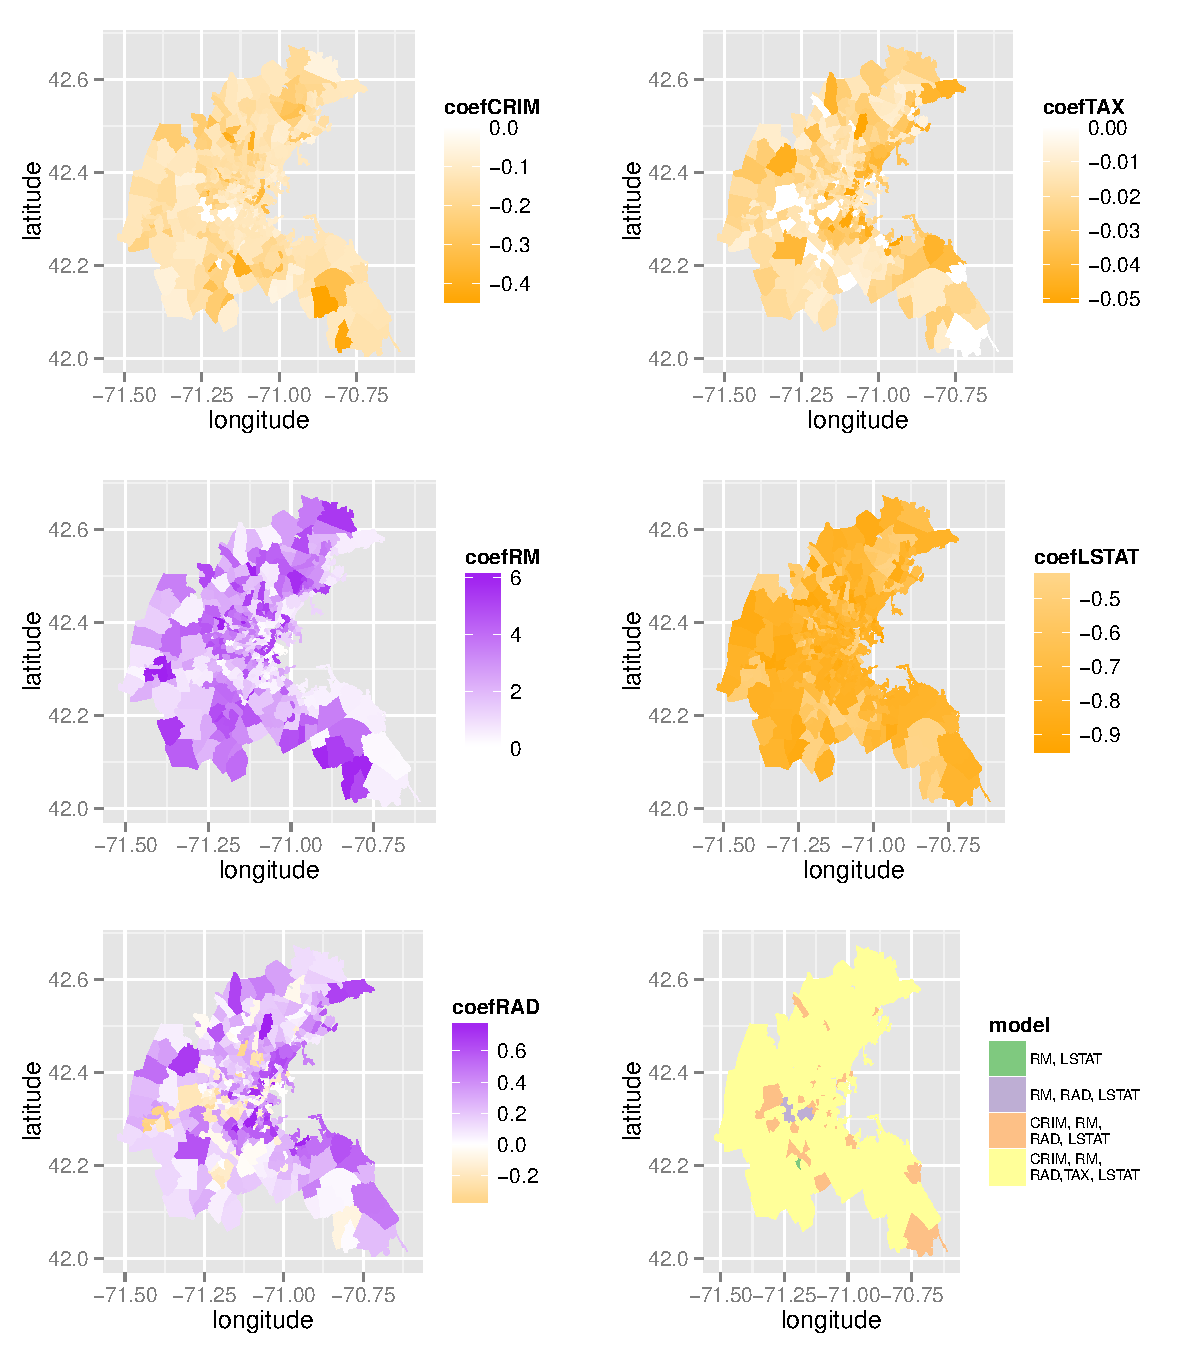
\includegraphics[width=\maxwidth]{figure/boston-plots} 
\caption{A varying coefficient regression model for the median house price in each census tract in Boston in 1970, estimated by local adaptive grouped regularization.
In the left column are the estimated coefficients for covariates CRIM (per-capita crime rate), RM (mean number of rooms per house), and RAD (an index of access to radial roads.
In the right column are the estimated coefficients for covariates TAX (property tax per $\$10,000$) and LSTAT (proportion of residents who are ``lower status"), and a map indicating which covariates were estimated to have nonzero coefficients in each census tract.
\label{fig:boston-lagr-coefs}}
\end{figure}

The estimates of the local coefficients are plotted in the first five panels of Figure \ref{fig:boston-lagr-coefs}.
The estimated coefficients of CRIM and LSTAT were everywhere negative or exactly zero, suggesting that the crime rate and proportion of ``lower-status" individuals were associated with a lower median house price. 
Meanwhile, the coefficient of RM was everywhere estimated to be positive, so the more rooms in the average house was everywhere associated with a higher median house price.
The coefficient of TAX was negative in most census tracts, but was estimated to be exactly zero in 50 tracts, indicating no discernable effect of the property tax rate on house prices in those tracts.
The coefficient of RAD is positive in some areas and negative
in others, indicating that the association of RAD with house prices is a local phenomenon.
The bottom right panel of Figure \ref{fig:boston-lagr-coefs} shows which covariates were estimated to have a nonzero coefficient in each tract.
There were 471 tracts where LAGR estimated that all the covariates had a nonzero coefficient, 43 tracts where all covariates except for TAX were estimated to have nonzero coefficients, six tracts where the coefficients of CRIM and TAX were estimated to be zero, and one tract where the coefficients of CRIM, RAD, and LSTAT were estimated to be zero.

\ifthenelse{\boolean{thesis}}{
An interesting result from the data example is the apparent relationship between the property tax rate and the coefficient of the TAX variable.
Of the $506$ Boston census tracts, there were $50$ where the estimated coefficient of the TAX variable was zero.
Four of those $50$ tracts ($8\%$) were locations where the property tax rate was at least $\$666$ per $\$10000$ (which encompasses the two highest property tax rates).
In total there were $137$ tracts where the property tax rate was at least $\$666$ per $\$10000$, which was $27\%$ of all tracts.
This suggests that the coefficient of the TAX variable was less likely to be zero in tracts with the highest property tax rates than in other tracts.
A rank sum test was used to test the null hypothesis that tracts where the coefficient of the TAX variable was estimated to be zero occurred independently of the property tax rate.
The alternative considered was that the tracts with an estimated zero TAX coefficient were clustered among the tracts with a lower property tax rate.
Of $1000$ uniform samples of size $50$ from the ranks of the property tax rates, only four had a smaller sum than that observed for the tracts where the TAX coefficient was estimated to be zero.
This provides evidence that the property tax rate was more likely to have no apparent effect on the median house price in tracts where the property tax was lower.}{}


% latex table generated in R 3.1.1 by xtable 1.7-4 package
% Wed Sep 24 17:10:32 2014

\section{Conclusions and Discussion \label{section-conclusion}}

We have developed a new method of LAGR and shown its oracle properties
for local variable selection and coefficient estimation in VCR models.
This innovation provides a natural and heretofore lacking flexibility to variable selection for
varying coefficient regression models, as any covariate may be included
in part of and not necessarily the entire domain of interest.
This is in contrast to the existing literature on variable selection
for VCR models that focuses on global variable selection, where a covariate is either 
included in or excluded from the model over its entire domain. Further,
the method of LAGR extends the adaptive group Lasso. In particular,
the previous literature on the adaptive group Lasso is insufficient
for local selection in a VCR model because the local weights are functions
of the kernel $K(\cdot)$ and the bandwidth $h$. As a result, the
local observation weights change with sample size and the coefficient
estimates converge at a slower rate than in the traditional adaptive
group Lasso.

\section*{References}
\bibliographystyle{chicago}
\bibliography{references}

\appendix

\section{Proofs of Theorems 1--2}
The results apply for a location parameter of arbitrary dimension, but the intended application was spatial analysis so the proofs proceed with $d=2$.
\subsection*{Proof of Theorem \ref{theorem:normality-glm}}
First, let $\bm{z}\in\mathbb{R}^{3p}$. Define the $q$-functions
to be the derivatives of the quasi-likelihood: $q_{j}(t,y)=\left(\partial/\partial t\right)^{j}Q\left(g^{-1}(t),y\right)$.
Then $q_{1}\left(\eta\left(s,\bm{z}\right),\mu\left(s,\bm{z}\right)\right)=\bm{0}$,
and $q_{2}\left(\eta\left(s,\bm{z}\right),\mu\left(s,\bm{z}\right)\right)=-\rho\left(s,\bm{z}\right)$.
Let 
\[
\tilde{\bm{\beta}}_{i}''=\left[\left(s_{i}-s\right)^{T}\left\{ \nabla^{2}\beta_{1}(s)\right\} \left(s_{i}-s\right),\dots,\left(s_{i}-s\right)^{T}\left\{ \nabla^{2}\beta_{p}(s)\right\} \left(s_{i}-s\right)\right]^{T}
\]
 be the $p$-vector of quadratic forms of location interactions on
the second derivatives of the coefficient functions.
\begin{proof}
Let $H'_{n}(\bm{u})=\mathcal{J}^{*}\left(\bm{\zeta}(s)+\alpha_{n}\bm{u}\right)-\mathcal{J}^{*}\left(\bm{\zeta}(s)\right)$
and $\alpha_{n}=h^{-1}n^{-1/2}$. Then, minimizing $H'_{n}(\bm{u})$
is equivalent to minimizing $H_{n}(\bm{u})$, where 
\begin{align*}
H_{n}(\bm{u}) &= - n^{-1}\sum_{i=1}^{n}Q\left(g^{-1}\left(\bm{Z}_{i}^{T}\left\{ \bm{\zeta}(s)+\alpha_{n}\bm{u}\right\} \right),Y_{i}\right)K\left(h^{-1}\|s-s_{i}\|\right)\\
 & + n^{-1}\sum_{i=1}^{n}Q\left(g^{-1}\left(\bm{Z}_{i}^{T}\bm{\zeta}(s)\right),Y_{i}\right)K\left(h^{-1}\|s-s_{i}\|\right)\\
 & +n^{-1}\sum_{j=1}^{p}\phi_{j}\left(s\right)\|\bm{\zeta}_{(j)}(s)+\alpha_{n}\bm{u}\|-\sum_{j=1}^{p}\phi_{j}\left(s\right)\|\bm{\zeta}_{(j)}(s)\|.
\end{align*}
Define
\[
\Omega_{n}=\alpha_{n}\sum_{i=1}^{n}q_{1}\left(\bm{Z}_{i}^{T}\bm{\zeta}(s),Y_{i}\right)\bm{Z}_{i}K\left(h^{-1}\|s-s_{i}\|\right)=\alpha_{n}\sum_{i=1}^{n}\omega_{i}
\]
and 
\[
\Delta_{n}= - \alpha_{n}^{2}\sum_{i=1}^{n}q_{2}\left(\bm{Z}_{i}^{T}\bm{\zeta}(s),Y_{i}\right)\bm{Z}_{i}\bm{Z}_{i}^{T}K\left(h^{-1}\|s-s_{i}\|\right)=\alpha_{n}^{2}\sum_{i=1}^{n}\delta_{i}.
\]
Then it follows from the Taylor expansion of $\mathcal{J}^{*}\left(\bm{\zeta}(s)+\alpha_{n}\bm{u}\right)$
around $\bm{\zeta}(s)$ that
\begin{align}
H_{n}\left(\bm{u}\right) &= -\Omega_{n}^{T}\bm{u}+(1/2)\bm{u}^{T}\Delta_{n}\bm{u}+\left(\alpha_{n}^{3}/6\right)\sum_{i=1}^{n}q_{3}\left(\bm{Z}_{i}^{T}\tilde{\bm{\zeta}}_{i},Y_{i}\right)\left[\bm{Z}_{i}^{T}\bm{u}\right]^{3}K\left(h^{-1}\|s-s_{i}\|\right)\nonumber \\
 & +\sum_{j=1}^{p}\phi_{j}\left(s\right)\left\{ \|\bm{\zeta}_{(j)}(s)+h^{-1}n^{-1/2}\bm{u}\|-\|\bm{\zeta}_{(j)}(s)\|\right\} .\label{eq:taylor-expanded-glm-criterion}
\end{align}
where $\tilde{\bm{\zeta}_{i}}$ lies between $\bm{\zeta}(s)$
and $\bm{\zeta}(s)+\alpha_{n}\bm{u}$. Since $q_{3}\left(\bm{Z}_{i}^{T}\tilde{\bm{\zeta}}_{i},Y_{i}\right)$
is linear in $Y_{i}$, $K\left(\cdot\right)$ is bounded, and, by
condition (C.6),
\[
\left(\alpha_{n}^{3}/6\right)E\left|\sum_{i=1}^{n}q_{3}\left(\bm{Z}_{i}^{T}\tilde{\bm{\zeta}}_{i},Y_{i}\right)\left[\bm{Z}_{i}^{T}\bm{u}\right]^{3}K\left(h^{-1}\|s-s_{i}\|\right)\right|=O\left(\alpha_{n}\right),
\]
the third term in (\ref{eq:taylor-expanded-glm-criterion}) is $O_{p}\left(\alpha_{n}\right)$.
The limiting behavior of the last term of (\ref{eq:taylor-expanded-glm-criterion})
differs between the cases $j\le p_{0}(s)$ and $j>p_{0}(s)$.
\emph{Case $j\le p_{0}(s)$:} If $j\le p_{0}(s)$, then $n^{-1/2}\phi_{j}(s)\to n^{-1/2}\lambda_{n}\|\bm{\zeta}_{(j)}(s)\|^{-\gamma}$
and $|\sqrt{n}\left\{ \|\bm{\zeta}_{(j)}(s)+\alpha_{n}\bm{u}_{(j)}\|-\|\bm{\zeta}_{(j)}(s)\|\right\} |\le h^{-1}\|\bm{u}_{(j)}\|$. Thus, 
\[
\lim\limits _{n\to\infty}\phi_{j}(s)\left(\|\bm{\zeta}_{(j)}(s)+\alpha_{n}\bm{u}_{(j)}\|-\|\bm{\zeta}_{(j)}(s)\|\right)\le\alpha_{n}\phi_{j}(s)\|\bm{u}_{(j)}\|\le\alpha_{n}a_{n}\|\bm{u}_{(j)}\|\to0
\]
\emph{Case $j>p_{0}(s)$:} If $j>p_{0}(s)$, then $\phi_{j}(s)\left(\|\bm{\zeta}_{(j)}(s)+\alpha_{n}\bm{u}_{(j)}\|-\|\bm{\zeta}_{(j)}(s)\|\right)=\phi_{j}(s)\alpha_{n}\|\bm{u}_{(j)}\|$.
Since $h=O(n^{-1/6})$, if $hn^{-1/2}b_{n}\xrightarrow{p}\infty$,
then $\alpha_{n}b_{n}\xrightarrow{p}\infty$. Now, if $\|\bm{u}_{(j)}\|\ne0$,
then 
\[
\alpha_{n}\phi_{j}(s)\|\bm{u}_{(j)}\|\ge\alpha_{n}b_{n}\|\bm{u}_{(j)}\|\to\infty.
\]
On the other hand, if $\|\bm{u}_{(j)}\|=0$, then $\alpha_{n}\phi_{j}(s)\|\bm{u}_{(j)}\|=0$.
By Lemma 1, $\Delta_{n}=\Delta+O_{p}\left(\alpha_{n}\right)$,
so the limit of $H_{n}(\bm{u})$ is the same as the limit of $H_{n}^{*}(\bm{u})$
where
\[
H_{n}^{*}(\bm{u})= -\Omega_{(a)n}^{T}\bm{u}_{(a)}+(1/2)\bm{u}_{(a)}^{T}\Delta_{(a)}\bm{u}_{(a)}+o_{p}\left(1\right)
\]
if $\|\bm{u}_{j}\|=0\;\forall j>p_{0}(s)$, and $H_{n}^{*}(\bm{u})=\infty$
otherwise. It follows that $H_{n}^{*}(\bm{u})$ is convex and has
a unique minimizer, called $\hat{\bm{u}}_{n}$. Let $\hat{\bm{u}}_{(a)n}$
$\Delta_{(a)}$ and $\Omega_{(a)n}$ be, respectively, the parts of
$\bm{u}_{n}$, $\Delta$, and $\Omega_{n}$ corresponding to the true
nonzero coefficients, and let $\hat{\bm{u}}_{(b)n}$ be the subvector
of $\hat{\bm{u}}_{n}$ corresponding to the true zero coefficients.
Then
\begin{align*}
\hat{\bm{u}}_{(a)n} &= \Delta_{(a)}^{-1}\Omega_{(a)n}+o_{p}\left(1\right)\text{ and }\hat{\bm{u}}_{(b)n}=\bm{0}
\end{align*}
by the quadratic approximation lemma \citep{Fan-Gijbels-1996}. By epiconvergence, the minimizer of the limiting function is the limit
of the minimizers $\hat{\bm{u}}_{n}$ \citep{Geyer-1994}.
Since $\Delta$ is a constant, the normality of $\hat{\bm{u}}_{(a)n}$
follows from the normality of $\Omega_{n}$, which is established
via the Cram\'{e}r-Wold device. Let $\bm{d}\in\mathbb{R}^{3p}$ be
a unit vector, and let
\[
\xi_{i}=q_{1}\left(\bm{Z}_{i}^{T}\bm{\zeta}(s),Y_{i}\right)\bm{d}^{T}\bm{Z}_{i}K\left(h^{-1}\|s_{i}-s\|\right).
\]
Then $\bm{d}^{T}\Omega_{n}=\alpha_{n}\sum_{i=1}^{n}\xi_{i}$. We establish
the normality of $\bm{d}^{T}\Omega_{n}$ by checking the Lyapunov
condition of the sequence $\left\{ \bm{d}^{T}Var\left(\Omega_{n}\right)\bm{d}\right\} ^{-1/2}\left\{ \bm{d}^{T}\Omega_{n}-\bm{d}^{T}E\Omega_{n}\right\} $.
By boundedness of $K\left(\cdot\right)$, linearity of $q_{1}\left(\bm{Z}_{i}^{T}\bm{\zeta}(s),Y_{i}\right)$
in $Y_{i}$, and conditions (C.6) and (C.8), we have that
\begin{equation}
n\alpha_{n}^{3}E\left(\left|\xi_{1}\right|^{3}\right)=O\left(\alpha_{n}\right)\to0.\label{eq:lyapunov-bound}
\end{equation}
We observe that (\ref{eq:lyapunov-bound}) implies that $n\alpha_{n}^{3}\left|E\left(\xi_{1}\right)\right|^{3}\to0$,
and since $E\left(\left|\xi_{1}-E\xi_{1}\right|^{3}\right)<E\left\{ \left(\left|\xi_{1}\right|+\left|E\xi_{1}\right|\right)^{3}\right\} \to0$,
the Lyapunov condition is satisfied. Thus, $\Omega_{n}$ asymptotically
follows a Gaussian distribution and the result follows from the quadratic
approximation lemma.
\end{proof}
\subsection*{Proof of Theorem \ref{theorem:selection-glm}}
\begin{proof}
The proof is by contradiction. Without loss of generality we consider
only the $p$th covariate group.
Assume $\|\hat{\bm{\zeta}}_{(p)}(s)\|\ne0$. Then $\mathcal{J}\left(\bm{\zeta}(s)\right)$
is differentiable w.r.t. $\bm{\zeta}_{(p)}(s)$ and is minimized
where 
\begin{align}
\phi_{p}(s)\hat{\bm{\zeta}}_{(p)}(s)\|\hat{\bm{\zeta}}_{(p)}(s)\|^{-1} &= \sum_{i=1}^{n}q_{1}\!\left(\bm{Z}_{i}^{T}\hat{\bm{\zeta}}(s),Y_{i}\right)\bm{Z}_{i(p)}K\left(h^{-1}\|s_{i}-s\|\right)\label{eq:glm-selection}
\end{align}
From Lemma 2, the right hand side of (\ref{eq:glm-selection})
is $O_{p}\left(1\right)$, so for $\hat{\bm{\zeta}}_{(p)}(s)$
to be a solution, we must have that $hn^{-1/2}\phi_{p}(s)\hat{\bm{\zeta}}_{(p)}(s)\|\hat{\bm{\zeta}}_{(p)}(s)\|^{-1}=O_{p}\left(1\right)$.
But since by assumption $\hat{\bm{\zeta}}_{(p)}(s)\ne\bm{0}$,
there must be some $k\in\{1,2,3\}$ such that $|\hat{\zeta}_{(p)_{k}}(s)|=\max\{|\hat{\zeta}_{(p)_{m}}(s)|:1\le m\le3\}$.
And for this $k$, we have that $|\hat{\zeta}_{(p)_{k}}(s)|\|\hat{\bm{\zeta}}_{(p)}(s)\|^{-1}\ge3^{-1/2}>0$.
Since $hn^{-1/2}b_{n}\to\infty$, we have that $hn^{-1/2}\phi_{p}(s)\hat{\bm{\zeta}}_{(p)}(s)\|\hat{\bm{\zeta}}_{(p)}(s)\|^{-1}\ge hb_{n}(3n)^{-1/2}\to\infty$
and therefore the left hand side of (\ref{eq:glm-selection}) dominates
the sum to the right side. Thus, for large enough $n$, $\hat{\bm{\zeta}}_{(p)}(s)\ne\bm{0}$
cannot maximize $\mathcal{J}\left(\cdot\right)$, and therefore $P\left\{ \hat{\bm{\zeta}}_{(b)}(s)=\bm{0}\right\} \to1$. 
\end{proof}

\section{Lemmas}
\begin{lem}
\label{lemma:omega}
\begin{multline*}
E\left[\sum_{i=1}^{n}q_{1}\left(\bm{Z}_{i}^{T}\bm{\zeta}(s),Y_{i}\right)\bm{Z}_{i}K_{h}\left(\|s-s_{i}\|\right)\right]=
\left(\begin{array}{c}
2^{-1}n^{1/2}h^{3}f(s)\kappa_{2}\bm{\Gamma}(s) \{\nabla^{2}\bm{\beta}(s) \}^{T}\\
\bm{0}_{2p}
\end{array}\right)+o_{p}\left(h^{2}\bm{1}_{3p}\right)
\end{multline*}
and
\begin{align*}
Var\left[\sum_{i=1}^{n}q_{1}\left(\bm{Z}_{i}^{T}\bm{\zeta}(s),Y_{i}\right)\bm{Z}_{i}K_{h}\left(\|s-s_{i}\|\right)\right] &= f(s){\rm diag}\left\{ \nu_{0},\nu_{2},\nu_{2}\right\} \otimes\bm{\Gamma}(s)+o\left(1\right)\\
&= \Lambda+o\left(1\right)
\end{align*}
\end{lem}

\begin{lem}
\label{lemma:delta}
\begin{align*}
E\left[\sum_{i=1}^{n}q_{2}\left(\bm{Z}_{i}^{T}\bm{\zeta}(s),Y_{i}\right)\bm{Z}_{i}\bm{Z}_{i}^{T}K_{h}\left(\|s-s_{i}\|\right)\right] &= -f(s){\rm diag}\left\{ \kappa_{0},\kappa_{2},\kappa_{2}\right\} \otimes\bm{\Gamma}(s)+o\left(1\right)\\
&= -\Delta+o\left(1\right)
\end{align*}
and
\[
Var\left\{ \left(\sum_{i=1}^{n}q_{2}\left(\bm{Z}_{i}^{T}\bm{\zeta}(s),Y_{i}\right)\bm{Z}_{i}\bm{Z}_{i}^{T}K_{h}\left(\|s-s_{i}\|\right)\right)_{ij}\right\} =O\left(n^{-1}h^{-2}\right)
\]
\end{lem}

The proofs are omitted.

\end{document}

